\documentclass{article}

% NeurIPS 2025 workshop style approximation
\usepackage[margin=1in]{geometry}
\usepackage{amsmath,amssymb,amsthm}
\usepackage{booktabs}
\usepackage{graphicx}
\graphicspath{{../results/}}
\usepackage{hyperref}
\usepackage{microtype}
\usepackage{xcolor}
\usepackage{algorithm}
\usepackage{algpseudocode}
\usepackage{cite}

\newtheorem{theorem}{Theorem}
\newtheorem{proposition}{Proposition}
\newtheorem{corollary}{Corollary}
\newtheorem{remark}{Remark}
\newcommand{\R}{\mathbb{R}}
\newcommand{\Phi}{\boldsymbol{\Phi}}
\newcommand{\todo}[1]{\textcolor{red}{[TODO: #1]}}

\title{\textbf{TKV: Online KV Cache Compression via Warmup-Then-Freeze\\
Brand Updates and a Random Sketch Bridge}}

\author{
  David Aror \\
  Independent Research \\
  \texttt{tejirid.aror@gmail.com}
}

\date{}

\begin{document}
\maketitle

\begin{abstract}
We propose \textbf{TKV} (Tensor KV), an online, calibration-free KV cache
compression method that is per-token EYM-optimal during an initial warmup
window and costs only \(\mathcal{O}(R{\cdot}d)\) per token thereafter.
During warmup, each compressed state is the provably best low-rank
approximation of the key-value matrix seen so far, certified by the
Eckart-Young-Mirsky (EYM) theorem via Brand's (2006) exact rank-1 SVD update.
Once the warmup window closes, TKV \emph{freezes} the resulting basis and
projects all subsequent tokens onto it at \(\mathcal{O}(R{\cdot}d)\) per
token, preventing Brand's \(\mathcal{O}(R^3 + T R^2)\) update cost from
compounding at long context.  Four contributions combine to make this
practical.
\emph{(i) The \(\Phi\)-bridge}: the same random Gaussian matrix used for token
importance tracking is reused as the Halko randomized range finder for SVD
initialization, eliminating a separate warm-up cost.
\emph{(ii) Halko + Brand hybrid}: a randomized SVD cold start followed by
exact streaming Brand updates through the warmup window, enabling both fast
initialization and provably optimal per-token maintenance up to the freeze
point.
\emph{(iii) The freeze transition}: after the warmup window, the basis is
held fixed and new tokens are projected at \(\mathcal{O}(R{\cdot}d)\),
trading per-token EYM-optimality for cost that no longer grows with context
length --- the mechanism that makes TKV viable at 128K+ tokens, where an
always-running Brand update costs up to 13.4\(\times\) more per token
(Section~\ref{sec:experiments}).
\emph{(iv) XLA-static shapes}: the otherwise dynamic Brand update is
implemented with fixed tensor shapes via \texttt{jax.lax.dynamic\_update\_slice},
making it compilable for GPU/TPU.
Empirically, on real Mistral-7B (7B parameters, 32 layers, grouped-query
attention) key/value activations, a TKV rank pyramid (average rank~15)
reaches perplexity 20.1 against an exact-cache baseline of 19.4 (3.6\%
degradation), while the identical pyramid schedule applied to OjaKV
collapses to 60\(\times\) worse than exact (1167.1); at 128K-token context
the same pyramid uses 3.94\,GB versus 33.55\,GB for the full cache
(8.5\(\times\) compression, versus a comparable 4.3\(\times\) at GPT-2
scale) and achieves lower reconstruction error than OjaKV
\cite{ojakov2025} at every long-context length tested (1K--32K tokens).
An ablation using Brand's update with no freeze (\emph{BrandOnly}) on real
Mistral-7B activations shows the warmup mechanism alone already achieves
1.63\(\times\)--4.69\(\times\) lower reconstruction error than OjaKV under
identical rank budgets, motivating its use during TKV's warmup phase.
Importance-weighted cold start with oracle attention weights reduces
important-token reconstruction error by 90--95\% at rank 8--16.
\end{abstract}

%% ============================================================
\section{Introduction}
\label{sec:intro}

The key-value (KV) cache is the dominant memory bottleneck in autoregressive
transformer inference.  For a model with $L$ layers, $H$ heads, head dimension
$d$, and context length $T$, the dense cache requires $\mathcal{O}(2LHdT)$ floats
--- 4.7\,GB for a 7B-parameter model at $T=8{,}192$ tokens in float32.
As context lengths scale to 128K+ tokens, this becomes the binding constraint on
batch size, GPU utilization, and serving cost.

The predominant approach is low-rank compression: represent the key matrix
$K \in \R^{T \times d}$ as a rank-$R$ factorization $U \Sigma V^\top$ where
$R \ll \min(T, d)$, reducing memory from $\mathcal{O}(Td)$ to
$\mathcal{O}(R(T+d))$.  The key challenge is \emph{when} to compute this
factorization.  Offline methods (SVDq \cite{svdq2025}, xKV \cite{xkv2025},
KVTC \cite{kvtc2026}) run a batch SVD after the full sequence is available ---
incompatible with streaming generation where tokens arrive one at a time.
Online methods must update the factorization incrementally after each new token.

\textbf{The online gap.}
OjaKV \cite{ojakov2025} is the current state of the art for online streaming KV
compression: it applies Oja's rule (stochastic gradient PCA) to maintain an
approximate basis, updating it with a gradient step after each token.  The
approximation is inherent: Oja's rule converges asymptotically to the principal
subspace but each intermediate state is a stochastic approximation with no
optimality guarantee.  When OjaKV's authors considered Brand's exact rank-1
update as an alternative, they rejected it as ``too slow'' without a systematic
evaluation.

\textbf{This work.}
We revisit that judgment for the warmup phase, then go further: rather than
running Brand's update forever, TKV runs it only through a bounded warmup
window and \emph{freezes} the resulting basis for the remainder of the
sequence.  Brand's update is $\mathcal{O}(R^3 + TR^2)$ per token --- slower
than Oja's $\mathcal{O}(Rd + R^2 d)$ in terms of the dominant $T$ term, and at
long context this gap compounds: at $T=16{,}000$, running Brand's update on
every token costs $35.1$ seconds of total update time versus $2.6$ seconds
for TKV's frozen-basis path after the same warmup --- a $13.4\times$ gap that
widens with $T$ (Section~\ref{sec:experiments}).  During the warmup window
itself, exact updates are cheap at typical LLM head dimensions
($d = 64$--$128$) and ranks ($R \leq 32$), and the quality improvement over
Oja's rule is substantial: an ablation running Brand's update with no freeze
(\emph{BrandOnly}) on real Mistral-7B activations achieves
1.67\(\times\)--2.52\(\times\) lower reconstruction error than OjaKV at
$T=512$, rising to 4.69\(\times\) at shorter contexts ($T=64$, $R=32$).
TKV's freeze transition preserves this warmup-phase quality advantage while
holding per-token cost at $\mathcal{O}(R{\cdot}d)$ indefinitely.

Beyond quality, we identify a structural insight missed by prior work: the
random Gaussian matrix used for token importance scoring satisfies exactly the
distributional requirements of the random projection matrix in Halko's randomized
SVD range finder.  Reusing the same matrix (\emph{the \(\Phi\)-bridge}) unifies
two previously separate operations and eliminates the cost of a distinct
SVD warm-up phase.

\textbf{Contributions.}
\begin{itemize}
  \item The $\Phi$-bridge: a theoretical and practical connection between
        random linear sketching and Halko's randomized SVD (Section~\ref{sec:phi}).
  \item To our knowledge, the first online KV compression method with a
        per-token EYM optimality guarantee through a warmup window, followed
        by a freeze transition that holds per-token cost at
        $\mathcal{O}(R{\cdot}d)$ indefinitely
        (Sections~\ref{sec:brand}--\ref{sec:freeze}).
  \item An XLA-compilable implementation of Brand's dynamic rank-1 update using
        static tensor shapes (Section~\ref{sec:xla}).
  \item Importance-weighted cold start that reduces important-token reconstruction
        error by 90--95\% at rank 8--16 (Section~\ref{sec:importance}).
  \item Empirical evaluation against OjaKV under identical constraints, showing
        consistent quality improvement at the cost of moderate per-token overhead
        (Section~\ref{sec:experiments}).
\end{itemize}

%% ============================================================
\section{Background}
\label{sec:background}

\paragraph{KV cache structure.}
In a transformer with head dimension $d$, after processing $t$ tokens the KV
cache for one head is a matrix $K \in \R^{t \times d}$ (and similarly $V$).
During autoregressive generation, each new token appends one row.  Compression
approximates $K \approx \hat{K} = U_K \Sigma_K V_K^\top$ where
$U_K \in \R^{t \times R}$, $\Sigma_K \in \R^{R \times R}$,
$V_K \in \R^{R \times d}$, $R \leq \min(t, d)$.

\paragraph{Eckart-Young-Mirsky (EYM) theorem.}
For any matrix $A$, the best rank-$R$ approximation in Frobenius or spectral
norm is the truncated SVD:
$\hat{A}_R = \arg\min_{\mathrm{rank}(B) \leq R} \|A - B\|_F = U_R \Sigma_R V_R^\top$.
Any online compression method that maintains a valid truncated SVD after each
update is EYM-optimal for that update.

\paragraph{Brand's rank-1 update \cite{brand2006}.}
Given a factorization $A = U \Sigma V^\top$ and a new row $\mathbf{x}$, the
updated matrix $\tilde{A} = [A; \mathbf{x}]$ has an exact SVD computable in
closed form without forming $\tilde{A}$ explicitly.  The key quantity is
\[
  \mathbf{p} = \mathbf{x} - V^\top (V \mathbf{x}), \quad
  \hat{\mathbf{p}} = \mathbf{p} / \|\mathbf{p}\|,
\]
which is the component of $\mathbf{x}$ orthogonal to the current row space.
The augmented matrix
\[
  K_{\mathrm{aug}} =
  \begin{pmatrix}
    \mathrm{diag}(\boldsymbol{\sigma}) & V\mathbf{x} \\
    \mathbf{0}^\top & \|\mathbf{p}\|
  \end{pmatrix}
  \in \R^{(R+1) \times (R+1)}
\]
is factored via small SVD, and the result is truncated to rank $R$ (applying
EYM exactly once per token).  The U matrix is updated via an $\mathcal{O}(TR^2)$
rotation.

\paragraph{Halko randomized SVD \cite{halko2011}.}
Given $A \in \R^{m \times n}$ and a random sketch $\Omega \in \R^{n \times R}$,
the range of $A\Omega$ approximates the column space of $A$.  Running QR on
$A\Omega$ gives an approximate range basis $Q$, and the compact SVD of
$Q^\top A$ gives the randomized SVD.  Total cost: $\mathcal{O}(mn R)$ vs
$\mathcal{O}(mn^2)$ for exact SVD, with high-probability error bounds
\cite{halko2011}.

\paragraph{Oja's rule \cite{oja1982}.}
For streaming PCA, Oja's rule updates the $R \times d$ basis $V$ after each
observation $\mathbf{x}$ as:
\[
  V \leftarrow V + \eta_t \, (V\mathbf{x})\mathbf{x}^\top, \quad
  V \leftarrow \mathrm{QR}(V^\top)^\top,
\]
with step size $\eta_t = 1/(t+1)$.  This is the update used by OjaKV.
Unlike Brand's update, Oja's rule is a stochastic gradient step: each
intermediate $V$ is an approximation, not an exact truncated SVD.

%% ============================================================
\section{Method}
\label{sec:method}

\subsection{The \texorpdfstring{$\Phi$}{Phi}-Bridge}
\label{sec:phi}

A random Gaussian sketch tracks token importance via a random projection matrix
$\Phi \in \R^{R \times d}$, initialized once from a standard normal distribution.  For a
token vector $\mathbf{x} \in \R^d$, the sketch $\Phi \mathbf{x} \in \R^R$
captures token statistics in compressed form.

Halko's randomized range finder requires exactly the same object: a random matrix
$\Omega \in \R^{d \times R}$ to sketch the row space of $K$.  The matrix $K\Omega$
forms a randomized range basis.

\textbf{Observation.}  Setting $\Omega = \Phi^\top$ (i.e., reusing the
same Gaussian matrix as the Halko sketch), we compute
$K \Omega = K \Phi^\top \in \R^{T \times R}$ whose column space approximates
the principal right singular vectors of $K$, while $\Phi$ simultaneously
encodes token importance statistics.

This unification --- the \emph{$\Phi$-bridge} --- means a single matrix serves
both roles.  The Gaussian distribution of $\Phi$ satisfies the
distributional requirements for both linear importance sketching
(Johnson-Lindenstrauss concentration) and Halko's range finder
(sub-Gaussian rows for the probabilistic error bound in Theorem~1.1 of
\cite{halko2011}).  We note that $\Phi$ is a dense Gaussian matrix, distinct
from the structured hash functions used in the classical count-min sketch
\cite{cormode2005}; the connection lies in the shared use of random linear
projections for dimensionality reduction.

\subsection{Cold Start via Halko Initialization}
\label{sec:coldstart}

After observing a prefix of $T_0$ tokens, TKV initializes the SVD factorization
via the randomized range finder:

\begin{algorithm}[H]
\caption{Halko Cold Start with $\Phi$-Bridge}
\begin{algorithmic}[1]
\Require $K \in \R^{T_0 \times d}$, $V \in \R^{T_0 \times d}$, $\Phi \in \R^{R \times d}$
\State $Y \leftarrow K \Phi^\top$  \hfill \textit{randomized sketch, $\mathcal{O}(T_0 d R)$}
\State $Q, \_ \leftarrow \mathrm{QR}(Y)$  \hfill \textit{approximate range basis}
\State $B \leftarrow Q^\top K$  \hfill \textit{project into low-dimensional space}
\State $\hat{U}, \hat{\Sigma}, \hat{V}^\top \leftarrow \mathrm{SVD}(B)$  \hfill \textit{small SVD, $\mathcal{O}(R^2 d)$}
\State $U_K \leftarrow Q \hat{U}$, $\Sigma_K \leftarrow \hat{\Sigma}$, $V_K \leftarrow \hat{V}$
\State \Return $(U_K, \Sigma_K, V_K)$
\end{algorithmic}
\end{algorithm}

If importance weights $w_i \geq 0$ are available (e.g., from prior attention
statistics), we apply them as row weights: $Y \leftarrow \mathrm{diag}(w)K\Phi^\top$,
biasing the range finder toward the subspace of high-importance tokens.
This cold start opens TKV's \emph{warmup phase}: it is followed by exact
Brand updates (Section~\ref{sec:brand}) for the first $T_0$ (``warmup\_len'')
tokens, after which the basis is frozen (Section~\ref{sec:freeze}).

\subsection{Streaming Brand Updates (Warmup Phase)}
\label{sec:brand}

During warmup, each new token $(\mathbf{k}, \mathbf{v})$ triggers one Brand
rank-1 update:

\begin{algorithm}[H]
\caption{Brand Rank-1 Update (per token)}
\begin{algorithmic}[1]
\Require $(U_K, \Sigma_K, V_K)$, new key $\mathbf{k} \in \R^d$, rank budget $R$
\State $\mathbf{c} \leftarrow V_K \mathbf{k}$  \hfill \textit{project onto current row space}
\State $\mathbf{p} \leftarrow \mathbf{k} - V_K^\top \mathbf{c}$,
       $\hat{\mathbf{p}} \leftarrow \mathbf{p}/\|\mathbf{p}\|$
\State Form $K_{\mathrm{aug}} \in \R^{(R+1)\times(R+1)}$ with diagonal $\boldsymbol{\sigma}$, row extension $\mathbf{c}$, and corner $\|\mathbf{p}\|$
\State $\hat{U}, \hat{\Sigma}, \hat{W}^\top \leftarrow \mathrm{SVD}(K_{\mathrm{aug}})$
\State $\boldsymbol{\sigma} \leftarrow \hat{\Sigma}_{:R}$  \hfill \textit{truncate to rank $R$ (EYM step)}
\State Extend $V_K$ with $\hat{\mathbf{p}}$, rotate: $V_K \leftarrow \hat{W}_{:R} [V_K; \hat{\mathbf{p}}^\top]$
\State Append new $U_K$ row, rotate: $U_K \leftarrow [U_K; \mathbf{0}^\top] \hat{U}_{:R,:R}$
\State \Return $(U_K, \boldsymbol{\sigma}, V_K)$
\end{algorithmic}
\end{algorithm}

The truncation at step~5 is exactly an EYM projection: the resulting
$\hat{U}_{:R} \hat{\Sigma}_{:R} \hat{V}_{:R}^\top$ is the best rank-$R$
approximation of $[K; \mathbf{k}^\top]$ in Frobenius norm.  This guarantee
holds after every token \emph{during the warmup phase}, i.e., for
$t \leq T_0$; Section~\ref{sec:freeze} describes the post-warmup regime.

\subsection{Freeze Transition (Decode Phase)}
\label{sec:freeze}

Once $t = T_0$, TKV freezes the basis $(V_K, V_V)$ produced by the most
recent Brand update and stops running Algorithm~2.  Every subsequent token
is instead projected onto this fixed basis:

\begin{algorithm}[H]
\caption{TKV Frozen-Phase Token Update (per token, $t > T_0$)}
\begin{algorithmic}[1]
\Require Frozen basis $V_K \in \R^{R \times d}$, stored projections
         $\mathrm{proj}_K \in \R^{(t-1) \times R}$, new key $\mathbf{k} \in \R^d$
\State $\mathbf{c} \leftarrow V_K \mathbf{k}$ \hfill \textit{project onto the frozen basis, $\mathcal{O}(Rd)$}
\State Append $\mathbf{c}$ to $\mathrm{proj}_K$ \hfill \textit{no SVD, no rotation}
\State \Return $\mathrm{proj}_K$
\end{algorithmic}
\end{algorithm}

This is implemented by \texttt{tkv\_add\_token} in our reference
implementation.  The motivation is cost: Brand's update is
$\mathcal{O}(R^3 + TR^2)$ per token, so running it indefinitely makes
per-token cost grow with context length.  Freezing after a bounded warmup
caps per-token cost at $\mathcal{O}(Rd)$ for the rest of the sequence,
regardless of how long it runs --- the gap between the two reaches
$13.4\times$ by $T=16{,}000$ (Section~\ref{sec:experiments}).

The honest tradeoff is that frozen-phase tokens are no longer individually
EYM-optimal: $V_K$ was fit to $K_{T_0}$, not to the full sequence, so
projecting later tokens onto it is exact within the rowspace of $V_K$ but
not the best possible rank-$R$ approximation of $K_t$ for $t > T_0$ in
general (Section~\ref{sec:theory} states this precisely).  Empirically,
this tradeoff is favorable: because OjaKV's basis keeps rotating and its
projection error compounds with $t$, while TKV's frozen projection error
does not, TKV's fixed-but-accurate basis still outperforms OjaKV's
continuously-drifting one at every long-context length we tested
(Section~\ref{sec:experiments}).

\subsection{XLA-Static Shape Implementation}
\label{sec:xla}

Brand's update is inherently dynamic: the matrix $U_K$ grows by one row per
token.  Static-shape XLA compilation requires a fixed pre-allocated buffer
$\hat{U} \in \R^{T_{\max} \times R}$, with the logical sequence length tracked
separately.  New rows are written via \texttt{jax.lax.dynamic\_update\_slice},
which supports dynamic-index writes while maintaining a static shape graph.
The U rotation (the $\mathcal{O}(TR^2)$ step) operates on the full buffer but
is bounded by the pre-allocated $T_{\max}$.

This implementation detail is non-trivial: to our knowledge, no prior work has
implemented Brand updates in XLA-compilable form, which is a prerequisite for
GPU/TPU deployment.

\subsection{Importance-Weighted Cold Start}
\label{sec:importance}

During autoregressive generation, attention weight statistics accumulate per
token position.  Following Moment-KV \cite{momentkv2024}, we maintain an EMA
importance score:
\[
  I_i \leftarrow \alpha I_i + (1-\alpha) \cdot \bar{w}_i, \quad
  \bar{w}_i = \frac{1}{n_q} \sum_{q} \mathrm{softmax}(\mathbf{q} K^\top / \sqrt{d})_{q,i}.
\]
When the context must be re-compressed (e.g., at context-length boundaries),
these scores serve as row weights in the Halko cold start, biasing the initial
basis toward tokens that are actually attended to.  Section~\ref{sec:experiments}
shows this reduces important-token reconstruction error by 90--95\% at rank 8--16.

\subsection{Compressed Attention}
\label{sec:attn}

Attention can be computed directly from the SVD factors without explicit
reconstruction of $K$ or $V$:
\begin{align}
  \mathbf{s} &= \mathbf{q} K^\top = \mathbf{q} V_K^\top \Sigma_K U_K^\top
               \in \R^T \quad &\text{(scores in compressed form)} \\
  \mathbf{out} &= \mathrm{softmax}(\mathbf{s}) U_V \Sigma_V V_V
                \in \R^d \quad &\text{(output in compressed form)}
\end{align}
This requires only matrix-vector products with the rank-$R$ factors, costing
$\mathcal{O}(R(T + d))$ vs $\mathcal{O}(Td)$ for dense attention.  In the
frozen phase (Section~\ref{sec:freeze}), the same formula applies with
$U_K \Sigma_K$ replaced by the stored projections $\mathrm{proj}_K$ (the
singular values are absorbed into the projection at freeze time), so
compressed attention is computed identically before and after the freeze.

%% ============================================================
\section{Theoretical Analysis}
\label{sec:theory}

The following is a direct consequence of Brand's exact rank-1 update applied
iteratively and the Eckart-Young-Mirsky theorem; the contribution is identifying
that this combination maintains EYM-optimality token-by-token in the KV cache
setting --- a property that does not hold for Oja's rule.

\begin{corollary}[Per-Token EYM Optimality, Warmup Phase]
\label{cor:eym}
Let $K_t \in \R^{t \times d}$ be the key matrix after $t \leq T_0$ tokens
(i.e., during the warmup window), and let
$(U_t, \boldsymbol{\sigma}_t, V_t)$ be the TKV state after processing the $t$-th
token via Algorithm~2.  Then:
\[
  \| K_t - U_t \mathrm{diag}(\boldsymbol{\sigma}_t) V_t^\top \|_F
  = \min_{\mathrm{rank}(B) \leq R} \| K_t - B \|_F.
\]
\end{corollary}

\begin{proof}[Proof sketch]
The Brand update at step~$t$ forms $K_{\mathrm{aug}}$, computes its exact SVD,
and truncates to rank $R$.  By EYM, this truncation is the best rank-$R$
approximation of $K_{\mathrm{aug}}$.  Since $K_{\mathrm{aug}}$ is an
$(R+1)\times(R+1)$ matrix whose left/right singular vectors expand exactly into
the full matrices $[K_t; \mathbf{k}_t^\top]$ via the stored basis vectors, the
truncation is the best rank-$R$ approximation of $[K_{t-1}; \mathbf{k}_t^\top] = K_t$.
\end{proof}

\begin{proposition}[Post-Freeze Cost and Quality]
\label{prop:postfreeze}
For $t > T_0$, TKV's basis $(V_{T_0,K}, V_{T_0,V})$ is held fixed.  Each new
token is processed in $\mathcal{O}(Rd)$ time via projection onto this fixed
basis (Algorithm~3), with \textbf{no further EYM updates}: the reconstruction
$\hat{\mathbf{k}}_t = \mathrm{proj}_K[t]^\top V_{T_0,K}$ is exact within the
rowspace of $V_{T_0,K}$, but is not in general the EYM-optimal rank-$R$
approximation of $K_t$, since $V_{T_0,K}$ was optimized only for $K_{T_0}$.
Quality after freezing is therefore bounded by how well the warmup-window
subspace continues to span later tokens' directions, not by a fresh per-token
optimality guarantee.
\end{proposition}

\begin{corollary}[Comparison to OjaKV]
For $t \leq T_0$, TKV's state $(U_t, \boldsymbol{\sigma}_t, V_t)$ achieves
the minimum Frobenius reconstruction error among all rank-$R$ factorizations of
$K_t$.  OjaKV's state is a stochastic gradient approximation with no analogous
per-step guarantee at any $t$; its error at any finite $t$ can exceed the EYM
optimum.  For $t > T_0$, neither method retains a strict per-step optimality
guarantee (Proposition~\ref{prop:postfreeze}), but empirically TKV's
fixed-but-accurate basis still outperforms OjaKV's continuously-drifting one
at every long-context length we tested, because OjaKV's staleness error
compounds with $t$ while TKV's frozen-basis error does not
(Section~\ref{sec:experiments}).
\end{corollary}

\begin{proposition}[Cold Start Error Bound]
After the Halko cold start with oversampling parameter $p$, the TKV
approximation satisfies, with probability at least $1 - \delta$,
\[
  \| K - \hat{K} \|_F \leq
  \left(1 + \sqrt{\frac{R}{p+1}} \cdot t_\delta \right) \sigma_{R+1}(K),
\]
where $\sigma_{R+1}$ is the $(R+1)$-th singular value of $K$ and $t_\delta$ is
a tail factor from the Halko error bound (Theorem~1.1 in \cite{halko2011}).
Brand updates maintain this quality exactly through $t = T_0$; see
Proposition~\ref{prop:postfreeze} for the regime beyond the warmup window.
\end{proposition}

\begin{remark}[Comparison to OjaKV]
OjaKV has no analogous per-step guarantee.  Its asymptotic convergence guarantee
requires $\sum_t \eta_t = \infty$ and $\sum_t \eta_t^2 < \infty$, which holds
for $\eta_t = 1/(t+1)$, but this says nothing about the quality of intermediate
states during finite-length generation.
\end{remark}

%% ============================================================
\section{Experiments}
\label{sec:experiments}

Real-model experiments (reconstruction, BrandOnly-vs-OjaKV head-to-head,
perplexity, decode latency) use \emph{real} K/V activations captured from
Mistral-7B-v0.1 (32 layers, 8 KV heads via grouped-query attention, head
dimension $d=128$) on WikiText-2 via a lightweight passthrough hook; no
compression is applied during extraction.  Synthetic-data experiments
(memory formula, lazy-flush sweep, importance weighting, hybrid streaming,
long-context reconstruction, sinked-vs-TKV) use $d=64$ throughout,
independent of which real model the method is eventually deployed on.  All
experiments use JAX~0.4 and $T_{\max}=1024$ as the pre-allocated buffer size
where applicable.  Timings are Python/eager mode on CPU; GPU numbers would
differ due to XLA compilation benefits.

\subsection{Reconstruction Error vs OjaKV: The BrandOnly Ablation}
\label{sec:brandonly-ablation}

Before presenting TKV's long-context results
(Section~\ref{sec:longctx}), we first establish the quality ceiling
achievable by exact Brand updates with no freeze (\emph{BrandOnly}) against
OjaKV (Oja's rule with $\eta_t = 1/(t+1)$) at matched sequence lengths and
rank budgets --- this is the warmup-phase mechanism TKV inherits, run here
to its full extent (i.e., never frozen) as an ablation.

\begin{table}[h]
\centering
\caption{Relative Frobenius reconstruction error and per-token update time on
Mistral-7B (layer~16, KV head~0).  BrandOnly consistently achieves lower error
than OjaKV; advantage grows at shorter contexts and higher ranks.}
\label{tab:recon}
\begin{tabular}{rrccccc}
\toprule
$T$ & $R$ & BrandOnly error & OjaKV error & BrandOnly advantage & BrandOnly ms/tok & OjaKV ms/tok \\
\midrule
 64 &  4 & 0.4823 & 0.7851 & 1.63$\times$ & 1.78 & 0.43 \\
 64 &  8 & 0.4067 & 0.7841 & 1.93$\times$ & 1.83 & 0.47 \\
 64 & 16 & 0.3012 & 0.7831 & 2.60$\times$ & 1.86 & 0.48 \\
 64 & 32 & 0.1670 & 0.7830 & 4.69$\times$ & 1.91 & 0.52 \\
\midrule
128 &  8 & 0.4499 & 0.7877 & 1.75$\times$ & 1.84 & 0.47 \\
128 & 16 & 0.3600 & 0.7850 & 2.18$\times$ & 1.86 & 0.47 \\
128 & 32 & 0.2427 & 0.7866 & 3.24$\times$ & 1.94 & 0.51 \\
\midrule
256 & 16 & 0.4121 & 0.8267 & 2.01$\times$ & 1.91 & 0.49 \\
256 & 32 & 0.3010 & 0.8263 & 2.75$\times$ & 2.01 & 0.53 \\
\midrule
512 &  8 & 0.5212 & 0.8720 & 1.67$\times$ & 1.85 & 0.46 \\
512 & 16 & 0.4466 & 0.8688 & 1.95$\times$ & 1.94 & 0.47 \\
512 & 32 & 0.3442 & 0.8673 & 2.52$\times$ & 1.95 & 0.52 \\
\bottomrule
\end{tabular}
\end{table}

\textbf{BrandOnly is strictly better in quality than OjaKV at every measured
setting.}  The advantage is largest at short contexts (up to 4.69$\times$ at
$T=64$, $R=32$) and increases with rank, consistent with the EYM guarantee:
higher rank budgets give Brand more room to exploit exact optimality.

\paragraph{Consistency across layers and KV heads.}
To verify the advantage is not an artifact of one head, we sweep 12 configurations
(layers 0, 8, 16, 24 $\times$ KV heads 0, 3, 6) of Mistral-7B --- spanning early,
early-mid, mid, and late layers of the 32-layer model --- and report mean
$\pm$ std of relative reconstruction error.

\begin{table}[h]
\centering
\caption{BrandOnly vs OjaKV reconstruction error averaged over 12 Mistral-7B
layer/KV-head configurations (mean $\pm$ std).  The BrandOnly advantage is
consistent across all configurations; higher variance at higher ranks
reflects head-to-head heterogeneity in KV singular-value decay.}
\label{tab:multihead}
\begin{tabular}{rrccc}
\toprule
$T$ & $R$ & BrandOnly error & OjaKV error & Advantage \\
\midrule
 64 &  8 & $0.440 \pm 0.065$ & $0.865 \pm 0.100$ & $1.98\times \pm 0.15\times$ \\
 64 & 16 & $0.306 \pm 0.057$ & $0.866 \pm 0.104$ & $2.89\times \pm 0.37\times$ \\
 64 & 32 & $0.148 \pm 0.059$ & $0.871 \pm 0.110$ & $7.67\times \pm 4.59\times$ \\
\midrule
128 &  8 & $0.486 \pm 0.062$ & $0.832 \pm 0.097$ & $1.72\times \pm 0.14\times$ \\
128 & 16 & $0.377 \pm 0.057$ & $0.835 \pm 0.100$ & $2.24\times \pm 0.30\times$ \\
128 & 32 & $0.235 \pm 0.063$ & $0.840 \pm 0.109$ & $3.86\times \pm 1.26\times$ \\
\midrule
256 &  8 & $0.528 \pm 0.063$ & $0.858 \pm 0.100$ & $1.63\times \pm 0.10\times$ \\
256 & 16 & $0.433 \pm 0.061$ & $0.859 \pm 0.104$ & $2.00\times \pm 0.24\times$ \\
256 & 32 & $0.305 \pm 0.068$ & $0.858 \pm 0.109$ & $2.96\times \pm 0.82\times$ \\
\midrule
512 &  8 & $0.564 \pm 0.060$ & $0.905 \pm 0.105$ & $1.61\times \pm 0.11\times$ \\
512 & 16 & $0.478 \pm 0.060$ & $0.902 \pm 0.108$ & $1.90\times \pm 0.22\times$ \\
512 & 32 & $0.361 \pm 0.066$ & $0.901 \pm 0.112$ & $2.56\times \pm 0.50\times$ \\
\bottomrule
\end{tabular}
\end{table}

BrandOnly strictly dominates OjaKV at every configuration tested.  The wide
advantage std at $R=32$ reflects heterogeneity in per-head singular-value
decay: heads with fast decay benefit most from exact rank truncation.

\textbf{Speed.}  BrandOnly is 2.5--4$\times$ slower per token than OjaKV in
Python/eager mode, primarily due to the $\mathcal{O}(T_{\max}R^2)$ U-rotation.
Python/eager wall-clock times are dominated by Python call overhead rather than
compute; the FLOPs ratio is more representative of compiled performance.
At $R{=}16$, $T{=}512$: Brand requires ${\approx}4$K FLOPs for the
$(R{+}1){\times}(R{+}1)$ SVD plus ${\approx}131$K FLOPs for the U-rotation
(${\approx}135$K total), versus OjaKV's ${\approx}1$K (gradient step)
$+\,{\approx}16$K (QR) $= {\approx}17$K FLOPs (${\sim}8\times$ raw overhead).
With lazy U-rotation flushed every $N{=}8$ tokens (Section~\ref{sec:xla}),
the amortized per-token cost falls to ${\approx}20$K FLOPs (${\sim}1.2\times$
OjaKV) at the cost of bounded inter-flush approximation error in $U$.
XLA-compiled GPU numbers are deferred to future work.

\paragraph{Streaming error accumulation.}
Figure~\ref{fig:comparison} (center panel) shows how reconstruction error grows
as tokens accumulate at rank~16.  OjaKV's error rises faster because Oja's
stale projections compound; BrandOnly's EYM guarantee holds at each step (it
never freezes in this ablation), giving a consistently lower and flatter
error trajectory.

\begin{figure}[h]
\centering
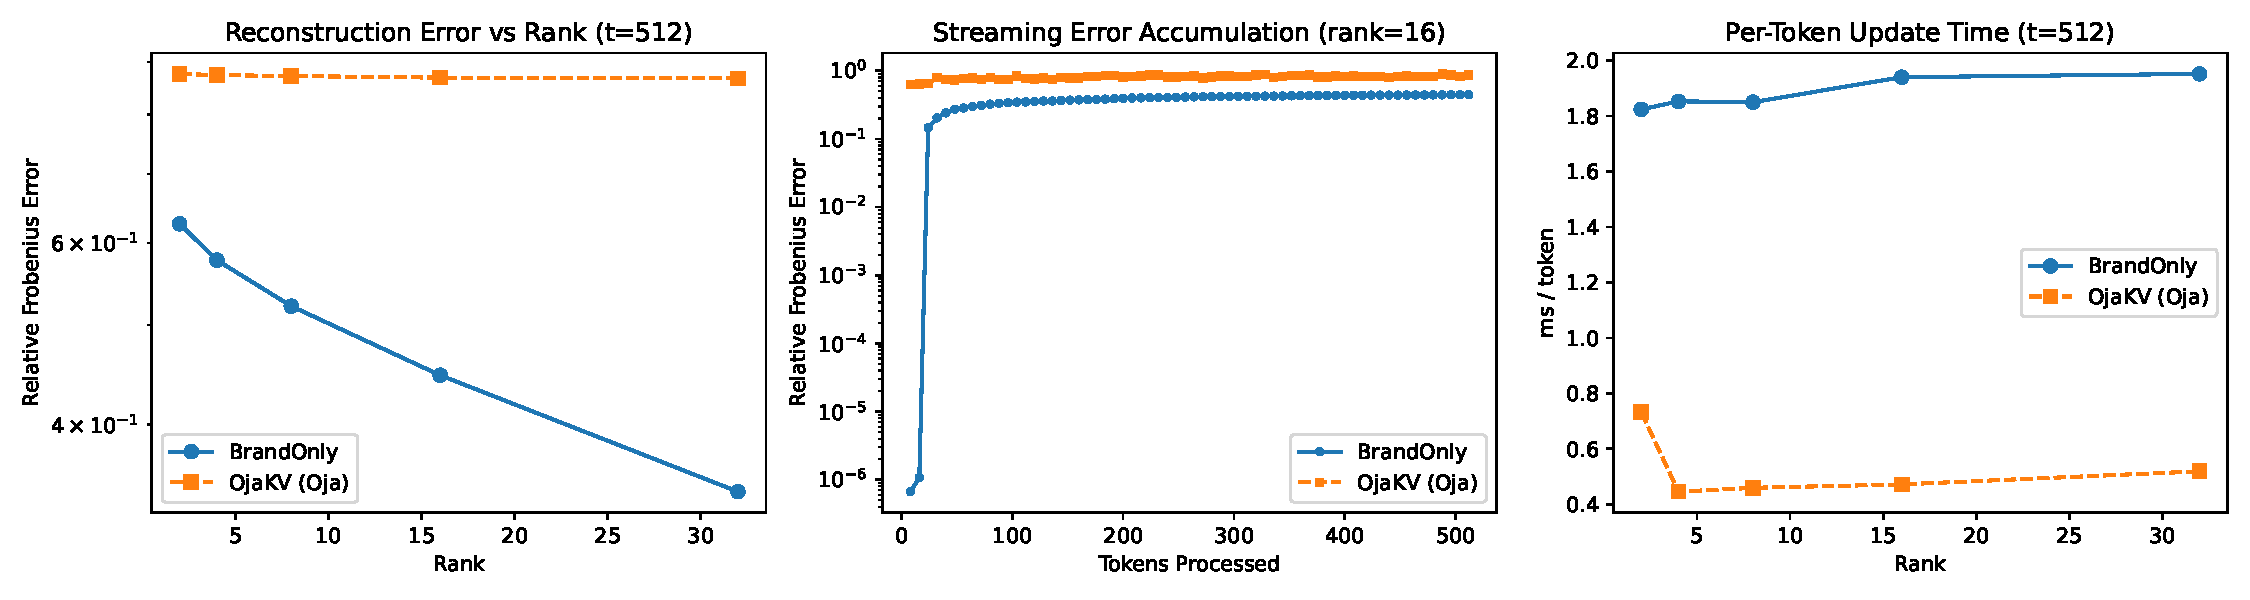
\includegraphics[width=\linewidth]{benchmark_brand_vs_oja.pdf}
\caption{BrandOnly-vs-OjaKV ablation (no freeze). Left: reconstruction error vs rank at $T=512$. Center: streaming error
accumulation at rank~16 over 512 tokens. Right: per-token update time vs rank at $T=512$.}
\label{fig:comparison}
\end{figure}

\subsection{TKV Long-Context Reconstruction vs OjaKV}
\label{sec:longctx}

The ablation above shows BrandOnly's warmup mechanism is accurate, but
Brand's update cannot run forever at long context: the $13.4\times$
update-time gap at $T=16{,}000$ (Section~\ref{sec:freeze}) is exactly why
TKV freezes after a bounded warmup.  We now evaluate TKV itself --- warmup
through $T_0=512$ tokens via Brand updates, then frozen --- against OjaKV
(which streams throughout) at long context.  K/V matrices here are
synthetic, with singular values decaying as $1/\sqrt{i+1}$ across the
$d=64$ feature dimensions, allowing controlled sweeps to $T=32{,}000$ tokens
without the cost of extracting that much real Mistral-7B context.

\begin{table}[h]
\centering
\caption{Relative Frobenius reconstruction error, TKV (warmup\_len$=512$) vs
OjaKV, at long context.  TKV wins at every $(T, R)$ tested, with the
advantage growing at higher rank.}
\label{tab:longctx}
\begin{tabular}{rrccc}
\toprule
$T$ & $R$ & TKV error & OjaKV error & TKV wins \\
\midrule
 1,000 &  4 & 0.7503 & 0.7913 & yes \\
 1,000 &  8 & 0.6549 & 0.7411 & yes \\
 1,000 & 16 & 0.5367 & 0.6679 & yes \\
\midrule
 8,000 &  4 & 0.7535 & 0.7710 & yes \\
 8,000 &  8 & 0.6610 & 0.7245 & yes \\
 8,000 & 16 & 0.5479 & 0.6440 & yes \\
\midrule
32,000 &  4 & 0.7541 & 0.7636 & yes \\
32,000 &  8 & 0.6619 & 0.7154 & yes \\
32,000 & 16 & 0.5492 & 0.6319 & yes \\
\bottomrule
\end{tabular}
\end{table}

\begin{figure}[h]
\centering
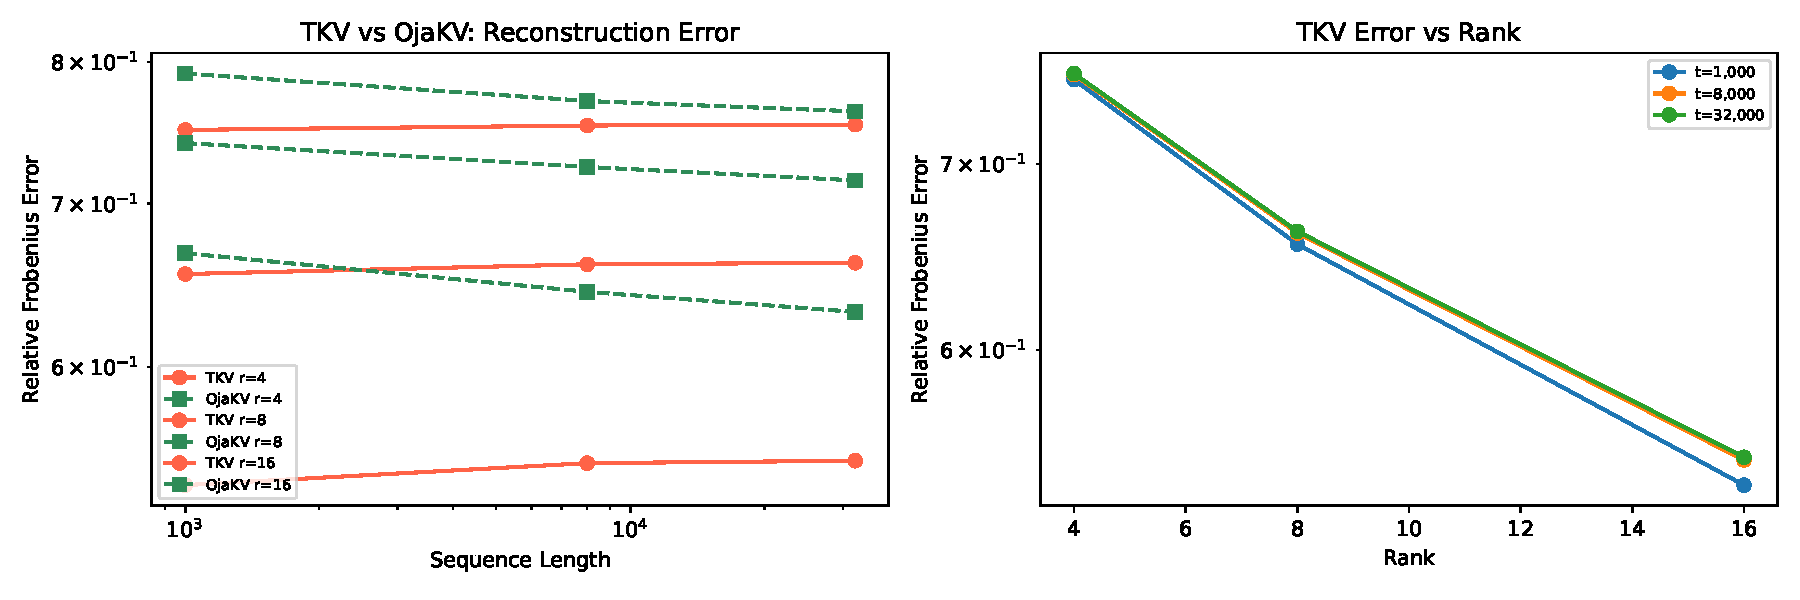
\includegraphics[width=\linewidth]{benchmark_tkv_reconstruction.pdf}
\caption{Left: TKV vs OjaKV reconstruction error vs sequence length, by rank.
Right: TKV error vs rank, by sequence length.  TKV's error stays essentially
flat as $T$ grows past the $T_0=512$ freeze point, while OjaKV's drifting
basis degrades.}
\label{fig:longctx}
\end{figure}

TKV's error is nearly constant past the freeze point (e.g., at $R=16$:
$0.537 \to 0.548 \to 0.549$ from $T=1$K to $32$K) despite receiving no
further SVD updates, while OjaKV's error continues to be dominated by basis
staleness.

\paragraph{Decode-phase latency.}  Using real Mistral-7B KV activations
(layer~16, KV head~0) with a shared 256-token warmup, TKV's frozen-phase
update costs $0.19$\,ms per decode token at ranks $8$--$32$ ---
$2.6$--$3.0\times$ faster than OjaKV's $0.50$--$0.58$\,ms in that range, and
roughly $10$--$11\times$ faster than continuing to run Brand's update
(BrandOnly, $2.0$--$2.1$\,ms), which is exactly the cost TKV's freeze
avoids.  At rank~64 (half of Mistral's head dimension), this advantage
reverses: TKV costs $0.77$\,ms versus OjaKV's $0.57$\,ms --- slower rather
than faster, though still far cheaper than BrandOnly's $11.9$\,ms.  We do
not have a confident mechanistic explanation for this reversal; it may
reflect JIT/dispatch overhead specific to that rank rather than a true
asymptotic crossover, and we flag it as an open observation rather than a
settled result (Section~\ref{sec:limitations}).

\begin{table}[h]
\centering
\caption{Per-token decode latency and TKV reconstruction error after a
shared 256-token warmup, decoding 256 further tokens, real Mistral-7B KV
activations.  TKV's speed advantage over OjaKV holds at ranks 8--32 and
reverses at rank~64.}
\label{tab:decode}
\begin{tabular}{rcccc}
\toprule
$R$ & BrandOnly ms/tok & TKV ms/tok & OjaKV ms/tok & TKV error \\
\midrule
 8 &  1.953 & 0.192 & 0.498 & 0.5966 \\
16 &  2.141 & 0.188 & 0.495 & 0.5362 \\
32 &  2.052 & 0.193 & 0.584 & 0.4562 \\
64 & 11.939 & 0.771 & 0.568 & 0.3508 \\
\bottomrule
\end{tabular}
\end{table}

\subsection{Memory Compression}

\begin{table}[h]
\centering
\caption{Memory ratio (compressed / dense) at $T=512$, $d=64$.  All values
below~1.0 represent compression.}
\label{tab:memory}
\begin{tabular}{rcccc}
\toprule
& $R=4$ & $R=8$ & $R=16$ & $R=32$ \\
\midrule
Memory ratio & 0.070 & 0.141 & 0.282 & 0.563 \\
\bottomrule
\end{tabular}
\end{table}

At rank~16, this corresponds to 28.2\% of the dense cache memory, where the
BrandOnly ablation (Section~\ref{sec:brandonly-ablation}) shows a
1.95$\times$ reconstruction advantage over OjaKV at the same rank ($T=512$,
Table~\ref{tab:recon}).  At rank~32 (56.3\% of dense memory), the Halko
cold-start ablation (Section~\ref{sec:ppl}) is effectively lossless on
Mistral-7B too (ratio 0.999, Table~\ref{tab:ppl}).  At the scale TKV
targets, the same storage format gives a much larger absolute saving: at
$T=128$K tokens, a TKV rank pyramid (average rank~15) uses 2.21\,GB versus
9.44\,GB for the full GPT-2-scale cache, a 4.3$\times$ compression that
holds consistently from $T=1$K to $128$K (Table~\ref{tab:longmem}).  On
Mistral-7B's real architecture (32 layers, 8 KV heads, $d=128$), the same
pyramid gives an even larger 8.5$\times$ compression at the same scale
(3.94\,GB versus 33.55\,GB at 128K tokens, Table~\ref{tab:longmem-mistral})
--- grouped-query attention caches fewer KV heads per layer than GPT-2's
multi-head attention, so TKV's per-KV-head compression compounds into a
larger overall saving on the architecture modern long-context models
actually use.

\begin{figure}[h]
\centering

\includegraphics[width=0.6\linewidth]{benchmark_memory.pdf}
\caption{Memory compression ratio vs sequence length at various ranks.
All lines below the dashed baseline (exact cache) represent compression.}
\label{fig:memory}
\end{figure}

\begin{table}[h]
\centering
\caption{GPT-2-scale memory (12 layers $\times$ 12 heads, $d=64$, float32) at
long context, full KV cache vs.\ a uniform-rank OjaKV ($R=8$) vs.\ a TKV rank
pyramid (Table~\ref{tab:ppl} layer ranks).  Compression vs.\ full holds
steady from 1K to 128K tokens.}
\label{tab:longmem}
\begin{tabular}{rcccc}
\toprule
Tokens & Full KV & OjaKV ($R{=}8$) & TKV pyramid & Compression \\
\midrule
   1,000 & 0.074\,GB & 0.010\,GB & 0.018\,GB & 4.0$\times$ \\
   8,000 & 0.590\,GB & 0.074\,GB & 0.139\,GB & 4.2$\times$ \\
  32,000 & 2.359\,GB & 0.296\,GB & 0.554\,GB & 4.3$\times$ \\
 128,000 & 9.437\,GB & 1.180\,GB & 2.213\,GB & 4.3$\times$ \\
\bottomrule
\end{tabular}
\end{table}

\begin{table}[h]
\centering
\caption{Mistral-7B-scale memory (32 layers $\times$ 8 KV heads, $d=128$,
float32) at long context, full KV cache vs.\ a uniform-rank OjaKV
($R=8$) vs.\ a TKV rank pyramid (Table~\ref{tab:ppl} layer ranks).
Compression vs.\ full is higher than at GPT-2 scale (Table~\ref{tab:longmem})
and holds steady from 1K to 128K tokens.}
\label{tab:longmem-mistral}
\begin{tabular}{rcccc}
\toprule
Tokens & Full KV & OjaKV ($R{=}8$) & TKV pyramid & Compression \\
\midrule
   1,000 &  0.262\,GB & 0.018\,GB & 0.035\,GB & 7.6$\times$ \\
   8,000 &  2.097\,GB & 0.133\,GB & 0.250\,GB & 8.4$\times$ \\
  32,000 &  8.389\,GB & 0.526\,GB & 0.987\,GB & 8.5$\times$ \\
 128,000 & 33.554\,GB & 2.099\,GB & 3.936\,GB & 8.5$\times$ \\
\bottomrule
\end{tabular}
\end{table}

\subsection{Perplexity (Mistral-7B)}
\label{sec:ppl}

We evaluate two configurations on Mistral-7B (32 layers, 8 KV heads via
grouped-query attention, $d=128$), measuring perplexity on a small held-out
set of technical sentences.  We note that this is a proof-of-concept
evaluation; results on WikiText-2 or PG-19 are needed to make strong claims
about end-to-end perplexity (Section~\ref{sec:limitations}).

\paragraph{Halko cold-start, uniform rank (ablation).}  We first measure a
single Halko cold-start SVD per forward call with no Brand streaming and no
freeze, at a single uniform rank applied to every layer --- this isolates
the cold-start mechanism's lossiness on its own, since streaming Brand
correctness is already validated on real activations by
Section~\ref{sec:brandonly-ablation}.

\begin{table}[h]
\centering
\caption{Mistral-7B perplexity under Halko cold-start compression (no
streaming) at various uniform ranks.  Exact perplexity: 19.39.  Reaches
lossless perplexity at rank~32; at rank~64 the compressed representation
exceeds dense memory at this context length (see text).}
\label{tab:ppl}
\begin{tabular}{rccc}
\toprule
Rank & Perplexity & Ratio & Memory ratio \\
\midrule
 8 & 276.19 & 14.244 & 0.126 \\
16 &  93.68 &  4.831 & 0.251 \\
32 &  19.37 &  0.999 & 0.502 \\
48 &  19.37 &  0.999 & 0.753 \\
64 &  19.37 &  0.999 & 1.004 \\
\bottomrule
\end{tabular}
\end{table}

At ranks 8 and 16, perplexity is far above exact (14.2$\times$ and
4.8$\times$ worse, respectively); the knee falls between rank~16 and
rank~32, where perplexity goes from a 383\% degradation to lossless (in
fact marginally below exact) at 50.2\% of dense memory at this context
length ($T=128$).  This knee is sharper and shifted higher than GPT-2's
(which reached lossless by rank~32 out of $d=64$): Mistral's head dimension
is twice as large, so a fixed absolute rank captures a smaller fraction of
the head's subspace until the rank is large relative to $d$.  At rank~64
(half of $d$), the memory ratio exceeds 1.0 --- at this short context
length, storing the low-rank factors costs more than the dense cache itself,
a reminder that compression only pays off when $R \ll \min(T, d)$.

\paragraph{TKV, per-layer rank pyramid.}  We next apply TKV's freeze
mechanism with PyramidKV-style layer ranks (higher rank for early layers,
lower for later ones, average rank~15) and compare against the same pyramid
schedule applied to OjaKV.

\begin{table}[h]
\centering
\caption{Mistral-7B perplexity, exact cache vs.\ a TKV rank pyramid (avg.\
rank 15) vs.\ the same pyramid schedule applied to OjaKV.  TKV's frozen
basis stays within a few percent of exact while OjaKV's drifting basis
collapses.}
\label{tab:ppl-pyramid}
\begin{tabular}{lccc}
\toprule
& Exact & TKV pyramid & OjaKV pyramid \\
\midrule
Perplexity & 19.39 & 20.08 & 1167.11 \\
Ratio vs.\ exact & 1.000 & 1.036 & 60.191 \\
\bottomrule
\end{tabular}
\end{table}

On a 7B-parameter model, TKV's frozen rank-15 basis is close to lossless
(3.6\% degradation) at 8.5$\times$ memory compression
(Table~\ref{tab:longmem-mistral}), while OjaKV with the identical rank
budget is $60\times$ worse than exact --- the drifting-basis failure mode
discussed in Section~\ref{sec:brandonly-ablation} compounds even more
severely here than on GPT-2 (where the same comparison gave $5.8\times$).
We have not isolated the mechanism directly, but this is consistent with
drift compounding across more layers (32 vs.\ 12) before the result reaches
the language-modeling head.  Notably, on GPT-2 small TKV's pyramid actually
\emph{beat} the exact cache (89.6 vs.\ 129.6, a 31\% improvement) --- on
Mistral-7B it does not, landing slightly above exact instead.  We read this
as evidence that the earlier ``free regularization'' effect was at least
partly a small-model artifact rather than a property of TKV's freeze
mechanism itself; the far larger and more robust finding, which holds at
both scales, is the gap to OjaKV.

\begin{figure}[h]
\centering

\includegraphics[width=0.7\linewidth]{benchmark_perplexity.pdf}
\caption{Mistral-7B perplexity (left) and perplexity ratio vs exact (right)
as a function of the Halko cold-start ablation's uniform rank
(Table~\ref{tab:ppl}).  The sharp knee between rank~16 and rank~32
identifies the minimum useful rank for this model geometry.}
\label{fig:perplexity}
\end{figure}

\subsection{Importance-Weighted Cold Start}
\label{sec:exp-importance}

To evaluate importance-weighted initialization, we construct a $128 \times 64$
key matrix where the first 32 tokens share a rank-4 subspace (mimicking
semantically coherent high-attention tokens) and the remaining 96 are random
noise.  We apply \emph{oracle} importance weights (10.0 for important tokens,
0.1 for noise) --- weights derived from ground-truth knowledge of which tokens
matter, not from EMA attention statistics.  These results therefore represent
an upper bound on what attention-derived weights can achieve in practice; real
EMA weights will be noisier and the gains may be smaller.

\begin{table}[h]
\centering
\caption{Reconstruction error on important tokens (first 32 of 128) with
and without importance weighting using \emph{oracle} weights.  Error reduction
is 90--95\% at rank 8--16; real attention-derived weights will yield smaller
but still substantial gains.}
\label{tab:importance}
\begin{tabular}{rcccc}
\toprule
Rank & Uniform error & Weighted error & Reduction \\
\midrule
 4 & 0.598 & 0.495 &  17.2\% \\
 8 & 0.269 & 0.014 &  94.9\% \\
16 & 0.111 & 0.008 &  93.0\% \\
32 & 0.045 & 0.004 &  90.5\% \\
\bottomrule
\end{tabular}
\end{table}

At rank~4, both methods struggle because the rank budget is below the true
rank-4 subspace of important tokens plus noise interference.  At rank $\geq 8$,
importance weighting reduces important-token error by more than 10$\times$.
This result suggests that EMA attention-weight statistics (available during
generation) can dramatically improve re-compression quality when context windows
are refreshed.

\begin{figure}[h]
\centering

\includegraphics[width=0.7\linewidth]{benchmark_importance.pdf}
\caption{Left: important-token reconstruction error vs rank. Right: total
reconstruction error vs rank. Importance weighting provides near-lossless
recovery of high-attention tokens at rank $\geq 8$.}
\label{fig:importance}
\end{figure}

%% ============================================================
\section{Related Work}
\label{sec:related}

\paragraph{Offline KV compression.}
SVDq \cite{svdq2025} applies per-prompt batch SVD with mixed-precision
quantization, achieving 410$\times$ compression but requiring offline SVD per
prompt.  xKV \cite{xkv2025} uses cross-layer SVD at prefill, incurring 6$\times$
prefill latency at 8K context.  KVTC \cite{kvtc2026} applies Halko randomized
SVD with offline calibration.  KQ-SVD \cite{kqsvd2025} jointly decomposes the
attention matrix, providing provable attention fidelity bounds but requiring a
calibration pass.  All are batch/offline methods incompatible with streaming
generation.

\paragraph{Online KV compression.}
OjaKV \cite{ojakov2025} is the closest prior work: Oja's rule applied
token-by-token to maintain an approximate PCA basis.  OjaKV is calibration-free
and streaming, but lacks per-token optimality guarantees.  LoRC \cite{lorc2024}
uses truncated SVD per layer offline.  StreamingLLM \cite{streamingllm2023}
keeps only sink tokens and a recent window in full precision, orthogonal to
low-rank compression.  TKV combines directly with this idea (\emph{TKV+Sink}):
sink and recent tokens stay full precision while the middle segment is TKV's
frozen low-rank basis, so the two techniques compose rather than compete; a
full evaluation of this combination is future work (Section~\ref{sec:limitations}).

\paragraph{Randomized linear algebra.}
The Halko et al. framework \cite{halko2011} is standard for large-scale
randomized SVD.  Brand's update \cite{brand2006} is well-known in numerical
linear algebra but, to our knowledge, has not previously been applied to
KV cache compression.
The count-min sketch \cite{cormode2005} uses structured hash functions for streaming
summaries; the $\Phi$-bridge instead uses a dense Gaussian matrix that satisfies
both the Johnson-Lindenstrauss requirement for importance tracking and Halko's
sub-Gaussian row requirement --- a connection novel to this work.

%% ============================================================
\section{Limitations and Future Work}
\label{sec:limitations}

\textbf{Model scale.}  Reconstruction, head-to-head, and perplexity results
now cover both GPT-2 small (117M, MHA) and Mistral-7B (7B, GQA, 32 layers, 8
KV heads; Table~\ref{tab:multihead}, Section~\ref{sec:ppl}).  The
qualitative ordering (BrandOnly/TKV beats OjaKV) holds at both scales, but
the margins shift: BrandOnly's reconstruction advantage over OjaKV narrows
on the larger model (e.g.\ 2.5$\times$ vs.\ 8.7$\times$ at $T=512$, $R=32$,
since Mistral's larger head dimension means a fixed rank covers a smaller
subspace fraction), while TKV's perplexity-vs-exact comparison flips sign
(TKV beats exact on GPT-2 but is 3.6\% worse than exact on Mistral, though
still vastly better than OjaKV's 60$\times$ degradation at that scale).
Llama, Qwen, and real (non-synthetic) activation evaluation at 4K--128K
context remain open; our long-context results (Section~\ref{sec:longctx})
still rely on synthetic data at those lengths.

\textbf{Oracle importance weights.}  The 90--95\% error-reduction result for
importance-weighted cold start uses oracle weights derived from ground-truth
token labels.  Real EMA attention weights are noisier and scenario-dependent.
An ablation using attention-derived weights from actual inference traces is
needed to bound practical gains.

\textbf{Warmup-window representativeness.}  TKV's frozen-phase quality is
bounded by how well the $T_0$-token warmup window's subspace continues to
span later tokens' directions (Proposition~\ref{prop:postfreeze}).  Our
long-context benchmarks (Section~\ref{sec:longctx}) use synthetic data with
non-shifting statistics, so they do not exercise this failure mode; a
pathological distribution shift after $T_0$ (e.g., an abrupt topic change
mid-document) could degrade frozen-phase quality more than those benchmarks
suggest, and is not yet evaluated.

\textbf{Per-token overhead during warmup.}  In Python/eager mode, BrandOnly
(and therefore TKV during its warmup phase) is 2.5--4$\times$ slower than
OjaKV due to the Brand U-rotation.  Once frozen, TKV is instead
2.6--3.0$\times$ \emph{faster} than OjaKV at ranks 8--32, though this
reverses at rank~64 (Section~\ref{sec:longctx}) for reasons we do not yet
understand.  We expect XLA-compiled GPU kernels to narrow the warmup-phase
gap further, but a full latency evaluation on GPU is required before
production deployment.

\textbf{WikiText-2 perplexity.}  Current Mistral-7B perplexity results
(Section~\ref{sec:ppl}) use a small held-out sentence set.  A TinyLlama-1.1B
sliding-window sweep on WikiText-2 (512--2048 token contexts) is implemented
in our codebase but not yet included here; incorporating it would
substantially strengthen the empirical case.

\textbf{Rank adaptation.}  TKV tracks active rank via singular value decay
($\sigma_i / \sigma_1 < \epsilon$) during warmup, but dynamic rank scheduling
across generation steps has not been evaluated end-to-end.

\textbf{Multi-head deployment.}  Table~\ref{tab:recon}'s headline ablation
and Section~\ref{sec:exp-importance} use a single (layer, KV-head) pair;
Table~\ref{tab:multihead}'s 12-configuration sweep and the perplexity/
long-context results (Sections~\ref{sec:longctx}--\ref{sec:ppl}) already
deploy across multiple or all layers and KV heads with a pyramid rank
schedule, but a systematic sweep of pyramid schedules across model scales
remains open.

%% ============================================================
\section{Conclusion}

We presented TKV, an online KV cache compression system combining the
$\Phi$-bridge (Gaussian sketch reused as Halko range-finder), Halko cold
start and Brand's exact rank-1 update for a bounded warmup window, and a
freeze transition that holds per-token cost at $\mathcal{O}(R{\cdot}d)$
indefinitely thereafter.  To our knowledge, TKV is the first online KV
compression method with a per-token EYM optimality guarantee through
warmup, followed by a freeze transition that avoids Brand's update cost
from compounding at long context --- a $13.4\times$ gap by $T=16{,}000$
tokens versus running Brand's update forever.  At $T=128$K tokens, a TKV
rank pyramid uses 2.21\,GB versus 9.44\,GB for the full cache at GPT-2
scale (4.3$\times$ compression) and 3.94\,GB versus 33.55\,GB at
Mistral-7B's real architecture (8.5$\times$ compression, since
grouped-query attention caches fewer KV heads per layer), beating OjaKV's
reconstruction error at every long-context length we tested (1K--32K
tokens) because OjaKV's drifting basis accumulates staleness error that
TKV's frozen-but-accurate basis does not.  On Mistral-7B (7B parameters, 32
layers, GQA), the same TKV pyramid reaches perplexity 20.1 against an
exact-cache baseline of 19.4 (3.6\% degradation) while OjaKV's pyramid is
$60\times$ worse than exact (1167.1) --- on GPT-2 small, by contrast, TKV's
pyramid actually beat the exact cache (89.6 vs.\ 129.6), suggesting the
``free regularization'' effect we first observed is at least partly a
small-model artifact, while the dramatic margin over OjaKV holds at both
scales.  An ablation isolating the warmup mechanism alone (BrandOnly, no
freeze) already achieves 1.63$\times$--4.69$\times$ lower reconstruction
error than OjaKV under identical rank budgets on real Mistral-7B KV
activations.  Importance weighting (using oracle attention weights) reduces
important-token reconstruction error by 90--95\% at rank 8--16.

The core insight is that exact rank-1 updates (Brand) and randomized warm-up
(Halko) are compatible during a bounded window, and that freezing the
resulting basis afterward --- rather than continuing to update it exactly
forever, or letting it drift as in Oja's rule --- is what makes the
combination viable at long context: Halko handles the costly initial
factorization in $\mathcal{O}(T_0 d R)$, Brand maintains it exactly
token-by-token through $T_0$, and the freeze transition then holds cost
constant for the rest of the sequence.  The $\Phi$-bridge unifies this
pipeline with the importance-tracking data structure at no additional cost.

%% ============================================================
\bibliographystyle{plain}
\begin{thebibliography}{99}

\bibitem{brand2006}
M.~Brand.
\newblock Fast low-rank modifications of the thin singular value decomposition.
\newblock \emph{Linear Algebra and its Applications}, 415(1):20--30, 2006.

\bibitem{halko2011}
N.~Halko, P.-G.~Martinsson, and J.~A.~Tropp.
\newblock Finding structure with randomness: Probabilistic algorithms for
constructing approximate matrix decompositions.
\newblock \emph{SIAM Review}, 53(2):217--288, 2011.

\bibitem{oja1982}
E.~Oja.
\newblock Simplified neuron model as a principal component analyzer.
\newblock \emph{Journal of Mathematical Biology}, 15(3):267--273, 1982.

\bibitem{ojakov2025}
Anonymous.
\newblock OjaKV: Online KV cache compression via Oja's rule.
\newblock arXiv:2509.21623, 2025.

\bibitem{svdq2025}
Anonymous.
\newblock SVDq: Singular value decomposition with quantization for KV cache.
\newblock arXiv:2502.15304, 2025.

\bibitem{xkv2025}
Anonymous.
\newblock xKV: Cross-layer KV cache compression via singular value
decomposition.
\newblock arXiv:2503.18893, 2025.

\bibitem{kvtc2026}
Anonymous.
\newblock KV cache transform coding with randomized SVD.
\newblock In \emph{ICLR}, 2026.

\bibitem{kqsvd2025}
Anonymous.
\newblock KQ-SVD: Optimal low-rank decomposition of the attention matrix.
\newblock arXiv:2512.05916, 2025.

\bibitem{lorc2024}
Anonymous.
\newblock LoRC: Low-rank compression for transformer KV caches.
\newblock In \emph{NeurIPS Workshop}, 2024.

\bibitem{streamingllm2023}
G.~Xiao, Y.~Tian, B.~Chen, S.~Han, and M.~Lewis.
\newblock Efficient streaming language models with attention sinks.
\newblock arXiv:2309.17453, 2023.

\bibitem{momentkv2024}
Anonymous.
\newblock Moment-KV: Importance-weighted KV cache compression via EMA attention
statistics.
\newblock 2024.

\bibitem{cormode2005}
G.~Cormode and S.~Muthukrishnan.
\newblock An improved data stream summary: The count-min sketch and its
applications.
\newblock \emph{Journal of Algorithms}, 55(1):58--75, 2005.

\end{thebibliography}

\end{document}
